\documentclass[12pt,fleqn]{article}\usepackage{../../common}
\begin{document}
Döndürme (Rotation) - 2

Herhangi Bir Eksen (Vektör) Etrafında Dönüş

Daha öne Rodriguez yöntemi ile yaptığımız döndürme yaklaşımını bir başka
teknikle göstereceğiz. Bulmak istediğimiz $\vec{n}$ etrafında $\theta$ dönüşü
yaptıracak bir matris, yani öyle bir matris $R(\vec{n},\theta)$ arıyoruz ki bu
matrisle $\vec{v}$ vektörünü sağdan çarpınca $\vec{v}'$ elde edilecek ve bu yeni
vektör $\vec{v}$ vektörünün $\vec{n}$ etrafında $\theta$ kadar dönmüş hali
olacak [1, sf. 142]. Yazının geri kalanında $\vec{v} = v$, $\vec{n} = n$.. 

$$
v' = v R(n,\theta)
$$

$R(n,\theta)$ matrisini türetmek için önce $v'$ vektörünü $v,n,\theta$ bazında
temsil etmeyi görelim. Ana fikir problemi $n$'ye dik olan düzlem üzerinde
çözmek, ki bu şekilde 3 boyutlu problemi 2 boyutlu bir probleme indirgemiş
oluyoruz. İndirgeme için $v$ vektörünü iki $v_\parallel$ ve $v_\perp$ vektörüne
ayıracağız, öyle ki $v = v_\parallel + v_\perp$. Sonra bu ki vektörü ayrıca
döndüreceğiz ve böylece onların toplamları da dönmüş olacak, yani $v' =
v'_\parallel + v'_\perp$. Buraya kadar gördüklerimiz Rodriguez yaklaşımına
benziyor.

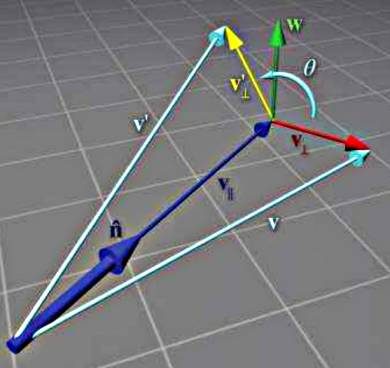
\includegraphics[width=10em]{phy_073_rot_01.jpg}

Tekniğin iyi tarafı $v_\parallel$ vektörü $n$ vektörüne paralel olduğu için $n$
etrafında dönüşten etkilenmez, o zaman sadece $v_\perp$ vektörünü döndürmek
yeterlidir, böylece $v' = v_\parallel + v'_\perp$ hesaplanabilir.

Hesap için şu adımları takip ediyoruz,

\begin{itemize}
   \item $v_\parallel$ vektörü $v$ nin $n$ ye paralel olan şeklidir, ya da
     $v$ vektörünün $n$ üzerinde yansıtılmış halidir [2], bu formülün
     $v_\parallel = (v \cdot n) n$ olduğunu biliyoruz.
   \item $v_\perp$ vektörü $v$ nin $n$ ye dik olan kısmıdır.
     $v = v_\parallel + v_\perp$ olduğu için $v_\perp = v - v_\parallel$.
   \item Üstteki şekilde $w$ vektörü var, bu vektör $v_\perp$ ve $v_\parallel$
     ile diktir, ve uzunluğu $v_\perp$ ile aynıdır. Bu vektör $v_\perp$
     vektörünü 90 derece döndürerek elde edilebilir. Bu sebeple $w = n \times v_\perp$.
     
\end{itemize}

Bu vektörlerle nasıl $v'$ hesaplayacağız? Dikkat edersek $w$ ve $v_\perp$ bir 2D
kordinate uzayı oluşturuyor. $v'_\perp$ vektörü $v'$ yi bu uzayda $\theta$ kadar
döndürerek elde edilebilir. Bu dönüşün formülünün

$$
v'_\perp = \cos \theta v_\perp + \sin \theta w
$$

olduğunu biliyoruz (ispatı bu anlatım ardından paylaşılıyor).

Şimdi eldeki formüllere bakalım:

$$
v_\parallel = (v \cdot n) n
$$

$$
v_\perp = v - v_\parallel
$$

$$
= v - (v \cdot n) n
$$

$$
w = n \times v_\perp
$$

$$
= n \times (v - v_\parallel)
$$

$$
= n \times v - n \times v_\parallel
$$

$n$ ve $v_\parallel$ birbirine paralel olduğu için çapraz çarpımları sıfırdır,

$$
= n \times v - 0 
$$

$$
w = n \times v
$$

$$
v'_\perp = \cos \theta v_\perp + \sin \theta w
$$

$$
= \cos \theta (v - (v \cdot n) n) + \sin \theta (n \times v)
$$

Üstteki değeri $v'$ formülü içine sokalım,

$$
v' = v'_\perp + v_\parallel
$$

$$
v' = \cos \theta (v - (v \cdot n) n) + \sin \theta (n \times v) + (v \cdot n) n
$$

\begin{minted}[fontsize=\footnotesize]{python}
import sys; sys.path.append('../phy_072_rot')
from mpl_toolkits.mplot3d import Axes3D
import plot3d

def rotate(v, n, theta):
    return np.cos(theta) * ( v - np.dot(v,n) ) + \
           np.sin(theta)* np.cross(n,v) + \
           np.dot(v,n)*n
 
o1 = np.array([5,5,5])
v1 = np.array([3,3,3])
n1 = np.array([-1/3.,2/3.,2/3.])

theta = np.deg2rad(20)

v1r = rotate(v1, n1, theta)

fig = plt.figure()
ax = Axes3D(fig)
plot3d.plot_vector(fig, o1, v1)
plot3d.plot_vector(fig, o1, v1r, 'cyan')
plot3d.plot_vector(fig, o1, 3*np.array(n1), 'red')
plot3d.plot_plane(ax, o1, n1, size=3)
ax.view_init(elev=40., azim=10)
plt.savefig('phy_073_rot_02.jpg')
\end{minted}

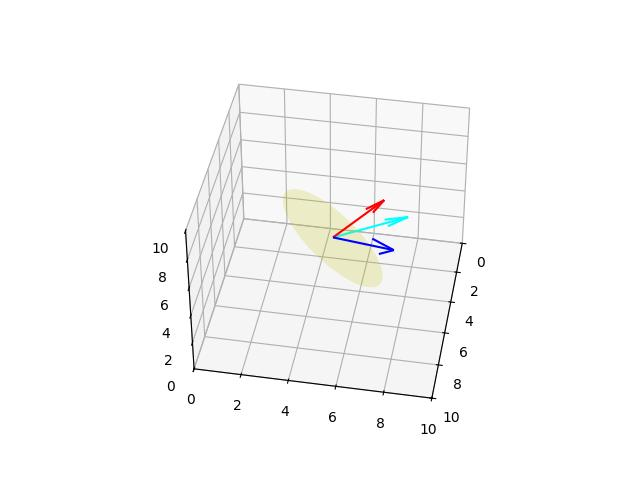
\includegraphics[width=20em]{phy_073_rot_02.jpg}

Teori

3D A,B vektörleri birbirine dikgen ve bir 2D uzay yaratıyorlar, ki sanki A
vektörü $x$ ekseni, B ise $y$ ekseni. A vektörünün $\theta$ açısı kadar
döndürülmesi $Y = \cos \theta A + \sin \theta B$ vektörünü verir (üstteki
problemde $A = v_\perp$, $B = w$).

İspat

A ve B 3D uzayında bir 2D düzlemi kapsayan iki dikgen vektör ise, A ve B'yi bu
2D düzlem için baz vektörleri olarak düşünebiliriz. A ve B tarafından kapsanan
düzlemdeki herhangi bir X vektörü, A ve B'nin bir doğrusal birleşimi olarak
ifade edilebilir:

$X = x_A A + x_B B$

Burada, $x_A$ ve $x_B$, X'in A ve B doğrultularındaki bileşenleridir.

A vektörü için, {A, B} bazındaki temsili, A doğrultusundaki bileşenin
1 ve B doğrultusundaki bileşenin 0 olduğu durumdur. Yani, A'yı bu 2D
baz sisteminde "x ekseni" ve B'yi "y ekseni" olarak düşünebiliriz,
burada A'nın "koordinatları" (1, 0) olur.

Şimdi, A vektörünü A ve B'nin kapsadığı düzlem içinde $\theta$ açısı
kadar döndürelim. Ortaya çıkan vektöre Y diyelim. Standart bir 2D
Kartezyen koordinat sisteminde, koordinatları $(x, y)$ olan bir vektör
$\theta$ açısı kadar saat yönünün tersine döndürüldüğünde, yeni
koordinatları $(x', y')$ şu şekilde bulunur:

$x' = x \cos \theta - y \sin \theta$

$y' = x \sin \theta + y \cos \theta$

Bizim durumumuzda, A vektörünün {A, B} bazındaki başlangıç
"koordinatları" $(1, 0)$'dır. A'yı $\theta$ kadar döndürdüğümüzde,
ortaya çıkan Y vektörünün {A, B} bazındaki yeni "koordinatları",
$(y_A, y_B)$, $(x, y) = (1, 0)$ kullanılarak 2D döndürme formülleriyle
bulunabilir:

$y_A = 1 \cdot \cos \theta - 0 \cdot \sin \theta = \cos \theta$

$y_B = 1 \cdot \sin \theta + 0 \cdot \cos \theta = \sin \theta$

Dolayısıyla, döndürülen Y vektörünün {A, B} bazındaki bileşenleri, A
doğrultusunda $\cos \theta$ ve B doğrultusunda $\sin \theta$ olur.

Şimdi Y vektörünü, bu bileşenleri kullanarak baz vektörler A ve B'nin
doğrusal birleşimi olarak yazabiliriz:

$Y = y_A A + y_B B$

$Y = \cos \theta A + \sin \theta B$

Bu, A vektörünün A ve B'nin kapsadığı 2D düzlem içinde $\theta$ açısı
kadar döndürülmesinin $Y = \cos \theta A + \sin \theta B$ vektörünü
verdiğini kanıtlar. Bu, bir 2D Kartezyen düzlemde x eksenindeki $(1,
0)$ vektörünün $\theta$ kadar döndürüldüğünde $(\cos \theta, \sin
\theta)$'ye dönmesiyle benzerdir. A ve B vektörleri, 3D uzayında bu 2D
dönüşüm için eksenleri sağlar.

[devam edecek]

Kaynaklar

[1] Dunn, {\em 3D Math Primer for Graphics and Game Development}

[2] Bayramlı, {\em Lineer Cebir - Giriş}

\end{document}




